%\documentclass[11pt]{article}
\documentclass[answers]{exam}

\usepackage{amsmath}
%\usepackage{extsizes}
\usepackage{amsmath,amssymb}
%\usepackage{omegavn,ocmrvn}
%\usepackage[utf8x]{inputenc}
\usepackage[utf8]{vietnam}
\DeclareUnicodeCharacter{00A0}{ }

\usepackage{longtable}
\usepackage{answers}
\usepackage{graphicx}
\usepackage{array}
\usepackage{pifont}
\usepackage{picinpar}
\usepackage{enumerate}
\usepackage[top=3.0cm, bottom=3.5cm, left=3.5cm, right=2.5cm] {geometry}
\usepackage{hyperref}


\newtheorem{bt}{Câu}
\newcommand{\RR}{\mathbb R}
\Newassociation{sol}{Solution}{ans}
\newtheorem{ex}{Câu}
\renewcommand{\solutionstyle}[1]{\textbf{ #1}.}


\begin{document}
% \noindent
\begin{tabular*}
{\linewidth}{c>{\centering\hspace{0pt}} p{.7\textwidth}}
Trường ĐHKHTN, ĐHQGHN & {\bf Học Kỳ 1 (2018-2019)}
\tabularnewline
K61 TTƯD & {\bf Bài Tập Giải Tích Số. No 1}
\tabularnewline
\rule{1in}{1pt}  \small  & \rule{2in}{1pt} %(Due date:)
\tabularnewline

%  \tabularnewline
%  &(Đề thi có 1 trang)
\end{tabular*}
%
%\Opensolutionfile{ans}[ans1]
\printanswers

\begin{bt} 
i) Hãy sử dụng phép làm tròn đến 3 chữ số thập phân để thực hiện các tính toán sau. Tính sai số tuyệt đối và sai số tương đối đến ít nhất 5 chữ số. 

\begin{tabular}{lll}
a. $133 + 0.921$ & b. $133 - 0.499$ & c. $(121 - 0.327) - 119$ \\
d. $(121 - 119) - 0.327$ & e. $\frac{\frac{13}{14}-\frac{6}{7}}{2e-5.4}$ & f. $-10 \pi + 6e - \frac{3}{62}$ \\
g. $\frac{2}{9} \cdot \frac{9}{7}$ & & h. $\frac{\pi-\frac{22}{7}}{\frac{1}{17}}$ \\
\end{tabular}
\vskip 0.2cm
ii) Câu hỏi tương tự nhưng sử dụng phép cắt 3 chữ số sau dấu chấm thập phân (giữ đúng 3 chữ số và 0 làm tròn).

%\begin{solution}
%	\begin{figure}[h!]
%		\centering
%		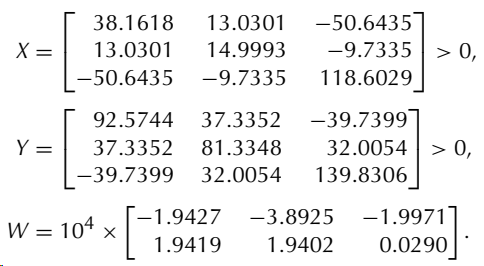
\includegraphics[width=0.7\linewidth]{Solution1/screenshot001}
%		\caption[Exercise 1.2.5, Burden-Faires, 8ed.]{}
%		\caption{}
%		\label{fig:screenshot001}
%	\end{figure}
%\end{solution}
\end{bt}

\begin{bt}
Ba số hạng khác không đầu tiên trong khai triển Maclaurin của hàm $arctan$ là $x - (1/3)x^3 + (1/5)x^5$. Hãy tính sai số tuyệt đối và sai số tương đối của $\pi$ bằng cách sử dụng đa thức đó để xấp xỉ hàm $arctan$ trong các biểu thức sau. Viết script để tính toán trong Matlab.
%
\begin{equation*} 
a.\ 4 \ (\arctan \frac{1}{2} + arctan \frac{1}{3}) \hskip 2cm b.\ 16 \ arctan \frac{1}{5} - 4 \ arctan \frac{1}{239}.
\end{equation*}
%
\end{bt}

\begin{bt}
Số $e$ được biểu diễn bởi công thức $e = \sum_{n=0}^{\infty}(1/n!)$. Hãy tính sai số tuyệt đối và tương đối sử dụng các xấp xỉ sau của $e$. Viết script để tính toán trong Matlab.
%
\[ 
a. \ \sum_{n=0}^{5}(1/n!) \qquad \qquad \qquad b. \ \sum_{n=0}^{10}(1/n!).
\] 
%
\end{bt}

\begin{bt}
Cho hàm số $f(x) = \frac{x cos x - sin x}{x - sin x}$. Viết script để tính toán trong Matlab các phần b, c, d.\\
a. Tìm $\underset{x \rightarrow 0}{\lim} f(x)$. \\
b. Sử dụng làm tròn đến 4 chữ số thập phân để tính $f(0.1)$. \\
c. Hãy thay thế các hàm lượng giác trong công thức của $f(x)$ bằng khai triển Maclaurin bậc 3 (chứa $x^3$) và thực hiện lại phần (b). \\
d. Cho giá trị chính xác của $f (0.1)=-1.99899998$. Xác định sai số tương đối của các xấp xỉ trong 2 phần (b) và (c).	
\end{bt}

\begin{bt}
Hãy sử dụng đa thức Taylor bậc $9$ của hàm $e^x$ và phép cắt 3 chữ số sau dấu chấm thập phân để xấp xỉ $e^{-5}$ bằng các xấp xỉ sau.
%
\[
a.\ e^{-5} \approx \sum_{n=0}^{9}((-5)^n/n!) \qquad \qquad \qquad b.\ e^{-5} = \frac{1}{e^5} \approx \frac{1}{\sum_{n=0}^{9}(5^n/n!)}. 
\]
%
c. Giá trị xấp xỉ của $e^{-5}$ đến 3 chữ số thập phân là $6.74e-3$. Công thức nào trong 2 công thức (a) và (b) cho ta giá trị xấp xỉ tốt hơn, vì sao?
\end{bt}

\centerline{———————————Hết——————————}

%\vspace{1cm}
%\noindent{\bf Chú ý:} {\it Cán bộ coi thi không giải thích gì thêm}\\
%\vspace{0.4cm}
%\noindent{\bf Họ và tên học sinh: \rule{3in}{.01pt} Lớp: \hrulefill}
%\Closesolutionfile{ans}
%\newpage
%\begin{center}
%{\LARGE{\bf ĐÁP ÁN}}
%\end{center}
%\begin{Solution}{1}
	\begin{figure}[h!]
		\centering
		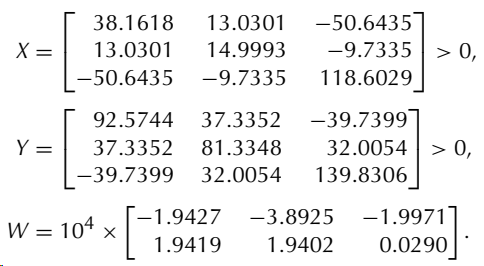
\includegraphics[width=0.7\linewidth]{Solution1/screenshot001}
		\caption[Exercise 1.2.5, Burden-Faires, 8ed.]{}
		\caption{}
		\label{fig:screenshot001}
	\end{figure}
\end{Solution}
 
   
\end{document}